\label{chapter:applications}

In this chapter we discuss applications of the improved binary XPFC model
introduced in Chapter \ref{chapter:improvements} to an application in
microstructure evolution.  We first begin with, we introduce  a
phenomenological set of equations of motion that describe solute and density
diffusion in the binary XPFC model. We then apply these to the examination of
the process of diffusion limited precipitation from solution.  Recent
experimental work on the precipitation of gold and silver nanoparticles
\cite{LOH17} and on the precipitation of calcium carbonate \cite{WALLACE13} has
demonstrated that the pathway to nucleation can deviate highly from the
approximations of Classical Nucleation Theory (CNT).  Specifically, both
experiments observe spinodal decomposition of the solution prior to nucleation
in the solute rich phase. In this chapter, we'll present early findings from
our new model that lend support for this dynamical behaviour and, additionally,
show that the growth behaviour post-nucleation may be more complex than usual
diffusive growth and coarsening typically observed.  To conclude we discuss
future applications both in the study of precipitation and other areas.

%%%%%%%%%%%%%%%%%%%%%%%
\subsection{XPFC Dynamics} %
%%%%%%%%%%%%%%%%%%%%%%%

To examine applications of our improvements to the XPFC model we begin by
considering equations of motion. Following \cite{GREENWOOD11_BINARY}, we use
conservative dynamics for both $n(x, t)$ and $c(x, t)$.
%
\begin{gather}
    \f{\partial n(x, t)}{\partial t} = 
        M_n \nabla^2\l(\f{\d \beta \Delta\F / \rho_0}{\d n(x, t)}\r) 
        + \xi_n(x, t), \\ 
    \f{\partial c(x, t)}{\partial t} = 
        M_c \nabla^2\l(\f{\d \beta \Delta \F / \rho_0}{\d c(x, t)}\r)
        + \xi_c(x, t),
\end{gather}
%
where $M_n$ and $M_c$ are the solute and density mobilities. The noise terms
$\xi_n(x, t)$ and $\xi_c(x, t)$ model thermal fluctuations. Their dynamics
follow the fluctuation-dissipation theorem, the theory of which is derived in
the Appendix \ref{appendix:noise}. These equations of motion are largely
phenomenological as, strictly speaking, there is no reason that the local
concentration should be conserved.  This conservation can be justified in the
limit that the total density does not deviate far from the reference. When this
is the case we have $c \equiv \B / \rho \approx \B / \rho_0$ which \textit{is}
conserved. For simplicity, we will carry out simulations in this chapter in
this limit.

%%%%%%%%%%%%%%%%%%%%%%%%%%%%%%%%%%%%%%%%%%%%%%%%%%%%%%%%%%%%%
\section{Multi-Step Nucleation of Nanoparticles in Solution} %
%%%%%%%%%%%%%%%%%%%%%%%%%%%%%%%%%%%%%%%%%%%%%%%%%%%%%%%%%%%%%

% Supply some background on the problem and motivation

Many nanoparticle solutions are formed by precipitation from solution and their
size distribution (polydispersity index) is of key importance to their
application. Therefore, a precise understanding of the kinetic pathway of
precipitation is of crucial importance in designing synthesis techniques of
highly mono-disperse nanoparticles.

As stated above, recent experimental work has shown that precipitation from a
solution can follow a pathway vary different from that assumed by Classical
Nucleation Theory (CNT) \cite{LOH17, WALLACE13}. CNT assumes that, for binary
systems, changes in composition occur simultaneously to changes in order. In
contrast, these experimental findings suggest that in certain systems changes
in composition can precede changes in order via spinodal decomposition. While
there is some dispute about whether or not to call this process a non-classical
\textit{nucleation} pathway \cite{DAVEY13, GEBAUER11}, the observed pathway to
precipitation raises several questions about its classification, regardless of
semantics.

%%%%%%%%%%%%%%%%%%%%%%%%%%%%%%%%%%%%%%%%%%%%%%%%%%%%%%%%%%%%%%
\subsection{Classical and Non-classical Nucleation Theories} %
%%%%%%%%%%%%%%%%%%%%%%%%%%%%%%%%%%%%%%%%%%%%%%%%%%%%%%%%%%%%%%

% Discuss classical nucleation theory

In CNT, the rate of formation of post-critical can be written as an Arrhenius
equation,
%
\begin{equation}
    J = \f{\partial n^*}{\partial t} = A e^{-\beta\Delta G^{\ddagger}},
\end{equation}
where,
\begin{description}[labelwidth=1cm, align=right]
    \item[$A$] is a constant prefactor,
    \item[$\Delta G^\ddagger$] is the Gibbs free energy of a critical nucleus
        and, 
    \item[$n^*$] is the number if critical nuclei.
\end{description}
% 
Following \cite{MYERSON04}, the probability of nucleation of a droplet of
volume $V$, $f_{nuc}(t)$, is then,
%
\begin{equation}
    f_{nuc}(t) = \mean{\f{N_{cry}}{N_{total}}} = 1 - e^{-J V t},
\end{equation}
%
where $N_{cry}$ and $N_{total}$ are the number of crystalline droplets and the
total number of droplets respectively.

% Discuss non-classical nucleation theory and the methods of reaction co-ordinates

CNT assumes that there is a single critical state which is specified by the
thermodynamic parameters of the target phase at a critical radius $R^*$. This
naive approach dramatically underestimate the time required to assemble a
critical nucleus due to its simplistic parametrization of the kinetic pathway
\cite{LUTSKO15, MYERSON04, MYERSON09}.

Improvements to CNT can be made to the model by increasing the parameter space
describing the nucleation process. Considering both radius and density of the
critical nucleus \cite{LUTSKO15} gives good agreement with nucleation of
globular proteins, for example. One problem with this approach is the selection
of appropriate parameters. There is no guarantee that a finite set parameters
will describe the kinetic pathway taken by a nucleus and if we are without a
fundamental technique for calculating the chosen parameters we have little way
of knowing if our theory is accurate or simply over-fit. In \cite{MYERSON09},
for example, nucleation data is fit to the functional form instead of using
calculated or otherwise measured parameters.

% Posit that field theory present an unbiased (un-parameterized) approach to nucleation

Statistical field theories such as the XPFC alloy model can help provide an
answer to this problem by taking an unbiased approach to nucleation process
within the context of CDFT.  The critical state, and entire kinetic pathway,
can be examined free of any particular parametrization. The equations of motion
can be integrated numerically for an ensemble systems and nucleation details
measured from the computed results.  Moreover, unlike other numerical
approaches to nucleation like molecular dynamics or formal density functional
theory, the PFC model can examine nucleation on diffusive time scales.

%%%%%%%%%%%%%%%%%%%%%%%%%%%%%%%%%%%%%%
\subsection{XPFC Modelling of Precipitation} %
%%%%%%%%%%%%%%%%%%%%%%%%%%%%%%%%%%%%%%

% Motivate a submerged spinodal phase diagram

To construct an appropriate free energy functional for a system analogous to
gold nanoparticles studied by Loh \textit{et al.} \cite{LOH17} we consider the
structure of its equilibrium phase diagram. Precipitation is indicative of a
simple liquid-solid coexistance curve. The presumed presence of spinodal
decomposition under certain circumstances indicates that is a metastable liquid
spinodal submerged beneath the liquid-solid coexistance curve \cite{DAVEY13}.
We assume that there must exist conditions under which the spinodal
decomposition of the metastable liquid phase occurs more rapidly than
nucleation directly from solution (ie., classical nucleation).

% Discuss the implementation of this phase diagram using our improvements

Producing a phase diagram in our XPFC model with these characteristics is very
similar to modelling a monotectic system with the exception that the spinodal
temperature $T_c$ must be low enough to hide the entire liquid spinodal below
the coexistance curve.  We will also centre the interpolation function
$\zeta_\alpha(c)$ about $c = 1$ so that the nanocrystalline solid $\alpha$ is
favoured at large concentration. The resulting density-density correlation
function for a 2 dimensional hexagonal precipitate would thus be,
%
\begin{equation}
    \label{eq:precip_corr}
    \tilde{C}_{nn}(k; c) = \exp\l\lbrace - \f{(c - 1)^2}{2\sigma_c^2}\r\rbrace
        \exp\l\lbrace \f{T}{T_0} \r\rbrace 
        \exp\l\lbrace - \f{(k - k_{10})^2}{2\sigma^2} \r\rbrace,
\end{equation}
%
where,
\begin{description}[labelwidth=1cm, align=right]
    \item[$\sigma_c$] is the width of the interpolation function
        $\zeta_\alpha(c)$, which controls the solvent solubility in the
        precipitate in this case and,
    \item[$k_{10}$] is the length of the [10] reciprocal lattice vector of the
        preciptate in equilibrium.
\end{description}

An example phase diagram of a system with sample parameters in equation
\ref{eq:precip_corr} is shown in figure \ref{fig:precip_phase_dia}. The
metastable binodal (coexistence) and spinodal curves are depicted below the
coexistence curve.

\begin{figure}
    \centering	
    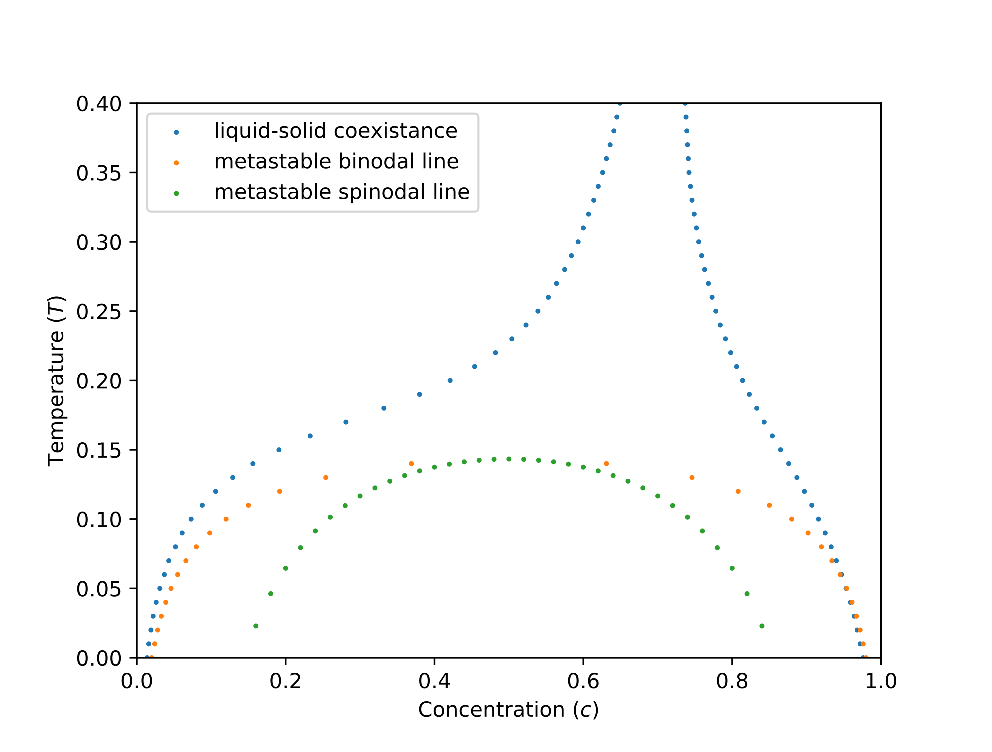
\includegraphics[scale=0.8]{solution.eps}
    \caption[Coexistance Phase Diagram with Metastable Spinodal]{
        \label{fig:precip_phase_dia} Phase Diagram of a Precipitating Solution
        with hexagonal $\alpha$ phase solid. The free energy parameters are
        $\eta = 2$, $\chi = 1$, $\omega=0.3$, $\epsilon_0=30$, $T_c = 0.15$ and
        $c_0 = 0.5$. The parameters for the correlation function from equation
        \ref{eq:precip_corr} are $\sigma = 0.8$, $k_{10} = 2\pi$, $T_0 = 1$ and
        $\sigma_c = 0.5$.
    }
\end{figure}

%%%%%%%%%%%%%%%%%%%%%%%%%%%%%%%%%%%%%%%%%%%%%%%%%%%%%%%%%%%%%%%%
\subsection{Dynamics of Precipitation: Results and Discussion} %
%%%%%%%%%%%%%%%%%%%%%%%%%%%%%%%%%%%%%%%%%%%%%%%%%%%%%%%%%%%%%%%%

% Describe with supporting figures the typical path way of precipitation.
 
We examined the precipitation process in a system that follows the XPFC model
with corresponding equilibrium phase diagram in figure
\ref{fig:precip_phase_dia}. The situation examined corresponded to a quench to
a temperature below the metastable spinodal curve. The spinodal curve marks an
inflection point in the liquid free energy meaning the metastable liquid
becomes fully unstable and decomposes into regions of differing concentration
as a result. A typical microstructure evolution sequence results for a typical
quench of a uniform solution of $c = 0.3$ from the liquid phase to a
temperature $T/T_0 = 0.07$ is shown in figure \ref{fig:precipitation}.
Frames (a)-(c) show the initial decmposition of the liquid, once below the
spinodal temperature, into two regions of high and low compositions. Frames
(d)-(f) show that once the concentration in the solute-rich regions of the
decomposed liquid occurs, nucleation of the solid phase begins to occur in
these confined liquid volumes. Once nucleated, the solid regions start/continue
to grow at the expense of the liquid phase. Finally, in frames (g)-(i), the
nucleated nanoparticles undergo growth and coarsening. This simulation is a
typical example where the nucleation of precipitates in preceded by spinodal
decomposition, which is consistent with the  the experimental findings
mentioned above for the nanoparticle and calcium carbonate systems \cite{LOH17,
WALLACE13}. While one simulation sequence is show here, this scenario was
typical of all ensembles we ran and from which we gathered statistics for the
data shown below. As mentioned above, we observed that once any solute-rich
regions crystallize, their growth is accelerated at the expense of
uncrystallized solute-rich regions. We refer to this phenomena as
\textit{sacrificial growth} (frames (d)-(f) in figure
\ref{fig:precipitation})). 
%
\begin{figure}
    \centering
    \begin{subfigure}[b]{0.3\textwidth}
        
\includegraphics[width=\textwidth]{initial}
        \label{fig:initial}
        \caption{}
    \end{subfigure}
    ~
    \begin{subfigure}[b]{0.3\textwidth}
        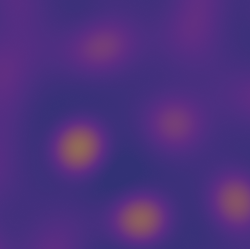
\includegraphics[width=\textwidth]{early_spinodal}
        \label{fig:early_spinodal}
        \caption{}
    \end{subfigure}
    ~
    \begin{subfigure}[b]{0.3\textwidth}
        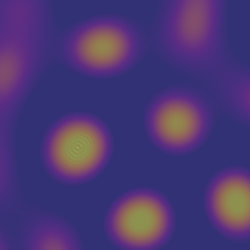
\includegraphics[width=\textwidth]{devel_spinodal.png}
        \label{fig:devel_spinodal}
        \caption{}
    \end{subfigure}

    \vspace{0.25cm}
    \begin{subfigure}[b]{0.3\textwidth}
        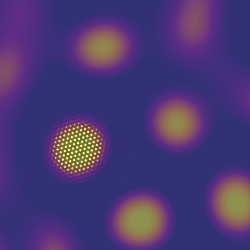
\includegraphics[width=\textwidth]{nucleation}
        \label{fig:nucleation}
        \caption{}
    \end{subfigure}
    ~
    \begin{subfigure}[b]{0.3\textwidth}
        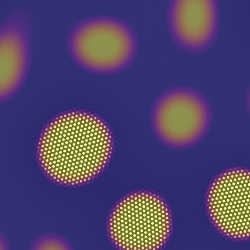
\includegraphics[width=\textwidth]{nucleation_and_sacrificial_growth}
        \label{fig:nucleation_and_growth}
        \caption{} 
    \end{subfigure}
    ~
    \begin{subfigure}[b]{0.3\textwidth}
        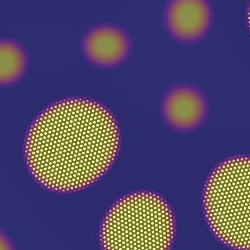
\includegraphics[width=\textwidth]{sacrificalgrowth}
        \label{fig:sacrifical_growth}
        \caption{}
    \end{subfigure}
    
    \vspace{0.25cm}
    \begin{subfigure}[b]{0.3\textwidth}
        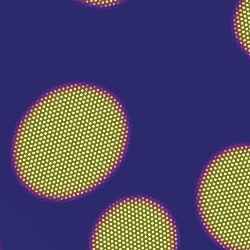
\includegraphics[width=\textwidth]{crystalgrowth}
        \label{fig:crystalgrowth}
        \caption{}
    \end{subfigure}
    ~
    \begin{subfigure}[b]{0.3\textwidth}
        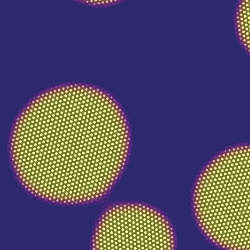
\includegraphics[width=\textwidth]{crystalgrowth2}
        \label{fig:crystalgrowth2}
        \caption{}
    \end{subfigure}
    ~ 
    \begin{subfigure}[b]{0.3\textwidth}
        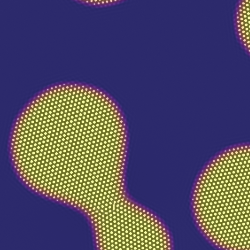
\includegraphics[width=\textwidth]{crystalgrowth3}
        \label{fig:crystalgrowth3}
        \caption{}
    \end{subfigure}
    \caption[Stages of precipitation of nanoparticles from solution]{
        \label{fig:precipitation}
        Various stages of precipitation of nanoparticles from solution. All
        thermodynamic parameters are shared with figure
        \ref{fig:precip_phase_dia}. The initial condition is a uniform solution
        quenched abruptly to $T$ = 0.07. The initial condition has
        concentration $c = 0.3$ and relative density is set to $n = 0.05$. Mobilities
        $M_n$ and $M_c$ are set to 1 and $W_c$ is set to 3.0. Numerical
        parameters are grid spacing $\Delta x = 0.125$ on a 1024 by 1024
        lattice with time step size $\Delta t = 0.0025$. Sub-figures (a) - (c)
        show spinodal decomposition of the liquid into solute right and solute
        poor regions. Sub-figures (d) - (f) show nucleation of the solid and
        solid growth at the expense of liquid regions.  The remaining
        sub-figures show only nanoparticle growth and coarsening.
    }
\end{figure}
%

% Discuss the growth picture (hyper / hypo diffusive)
%
To quantify the phenomena shown in figure \ref{fig:precipitation}, we examine
the mean radius $\mean{R(t)}$ of solute-rich domains as a function of time, and
average the results over an ensemble of 120 quenches analogous to those shown in 
figure \ref{ig:crystalgrowth3}. Here we define the mean
radius as the square root of the mean area,
%
\begin{equation}
    \mean{R(t)} = \sqrt{\mean{A(t)}}.
\end{equation}
%
The results obtained are not expected to depend on the precise definition of
$R(t)$.

In purely diffusive growth the mean radius should scale as $\mean{R(t)} \sim
t^{1/2}$, while at the late steges of growth, where coarsening occurs, the
growth rate is expected to follow  $\mean{R(t)} \sim t^{1/3}$ dynamics.  In
figure \ref{fig:scaling} we plot $\langle R(t)\rangle$ on a log-log graph.
Lines corresponding to the diffusive growth exponent are also drawn for
comparison to numerical results. The data shows that for early times,
crystalline regions grow at a hyper-diffusive rate. 
%
\begin{figure}
    \centering
    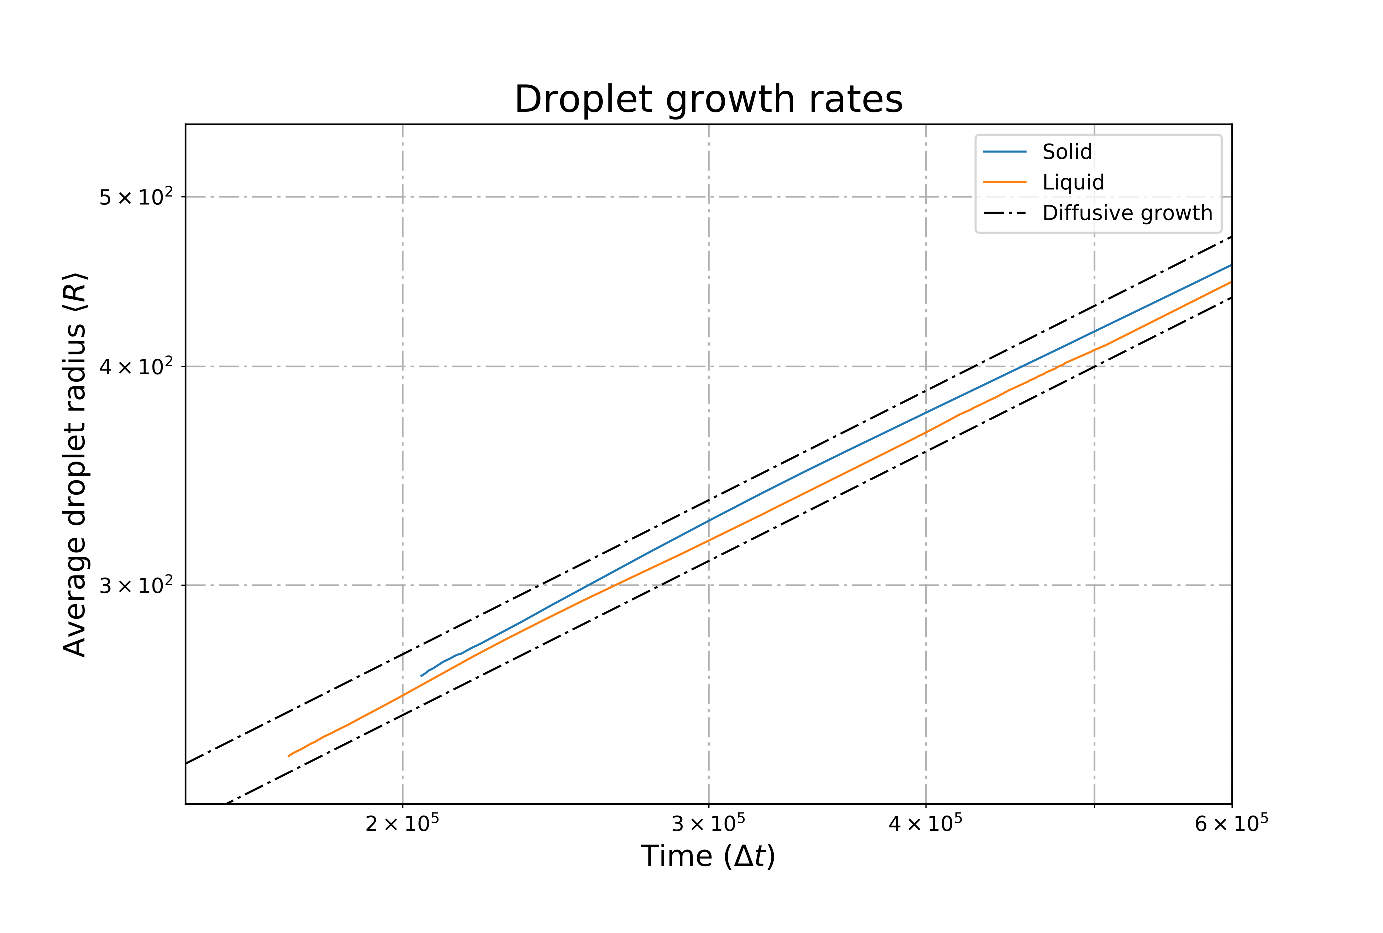
\includegraphics[width=\textwidth]{scaling}
    \caption{
        \label{fig:scaling}
        Droplet growth $\langle R(t) \rangle$ Versus time. Black line show
        $\sim t^{1/2}$ growth. Insets show early hyper-diffusive growth
        of crystalline nanoparticles and late stage hypo-diffusive growth.
    }
\end{figure}
%
\noindent This decays to hypo-diffusive after uncrystallized regions have disappeared and
coarsening takes over the kinetics of precipitation.

% Discuss the nucleation picture (fraction of uncrystallized droplets)
% and compare with MYERSON for example

During sacrificial growth period referred to above, we observe that nucleation
is suppressed in the remaining uncrystallized solute-rich regions. When both
crystallized and uncrystallized solute-rich regions exist, solute is segregated
into crystallized regions because of the difference in chemical potential.
Constricted by surface tension and deprived of solute, these remaining droplets
have a far slower nucleation rate (thermodynamic driving force) than when no
crystallized regions exist. This can be seen more quantitatively by examining
the fraction of uncrystallized droplets versus time. This is shown in figure
\ref{fig:incubation} for the case corresponding to the data in figure
\ref{fig:precipitation}. At $\sim 50\%$ crystallization, we see a pronounced
reduction in the nucleation rate as the diffusive process of sacrificial growth
dominates, consistent with our expected hypothesis above.
%
\begin{figure}
    \centering
    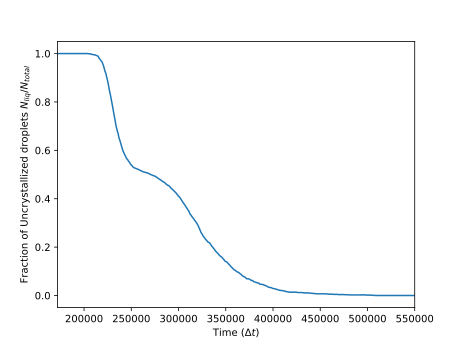
\includegraphics[width=1.0\textwidth]{incubation}
    \caption[Fraction of uncrystallized droplets in time]{
        \label{fig:incubation}
        Fraction of uncrystallized droplets in time.
    }
\end{figure}

%%%%%%%%%%%%%%%%%%%%%%%%%%%%%%%%%%%%%%%%%%%%%%%
\section{Outlook and Future Applications} %
%%%%%%%%%%%%%%%%%%%%%%%%%%%%%%%%%%%%%%%%%%%%%%%

% Explore the remainder of the phase space of nucleation
% Is CNT valid on some regime?
% Is the turnbull model valid elsewhere?

The results presented here describe the behaviour of a quench followed by
multi-step precipitation process of relevance to the precipitation of gold
nano-particles observed in recent experiments. The is noteworthy that the
predicted results were done within a single framework and set parameters
corresponding to the improved XPFC alloy model introduced in this thesis. The
dynamical results shown here point to a richness in the landscape of kinetic
pathways to precipitation. One direction for future application of the improved
XPFC framework is to explore more of this landscape and to determine the effect
of quench parameter and solution concentration in nucleation kinetics, as well
as the polydispersity of precipitated particles, key features of interest to
experimental investigations of this topic.

